\documentclass[aspectratio=169]{beamer}
\usepackage{ctex, hyperref}
\usepackage[T1]{fontenc}

% other packages
\usepackage{latexsym,amsmath,xcolor,multicol,booktabs,calligra}
\usepackage{graphicx,pstricks,listings,stackengine}
\renewcommand{\figurename}{Figure.}
\renewcommand{\tablename}{Table.}

\author{Kelompok 2}
\title{Analisis Kestabilan dan Bifurkasi Model Oregonator \\ dari Reaksi Kimia Belousov–Zhabotinsky}
\subtitle{\textit{Mini Project} Sistem Dinamik}
%\institute{Departemen Matematika \\ Universitas Gadjah Mada}
\date{Juni 2024}
\usepackage{sisu}

% defs
\def\cmd#1{\texttt{\color{red}\footnotesize $\backslash$#1}}
\def\env#1{\texttt{\color{blue}\footnotesize #1}}
\definecolor{deepblue}{rgb}{0,0,0.5}
\definecolor{deepred}{rgb}{0.6,0,0}
\definecolor{deepgreen}{rgb}{0,0.5,0}
\definecolor{halfgray}{gray}{0.55}

\lstset{
    basicstyle=\ttfamily\small,
    keywordstyle=\bfseries\color{deepblue},
    emphstyle=\ttfamily\color{deepred},    % Custom highlighting style
    stringstyle=\color{deepgreen},
    numbers=left,
    numberstyle=\small\color{halfgray},
    rulesepcolor=\color{red!20!green!20!blue!20},
    frame=shadowbox,
}


\begin{document}

\begin{frame}
    \titlepage
    \begin{figure}[htpb]
        \begin{center}      
\includegraphics[width=0.15\linewidth]{pic/logo_ugm.jpg}
        \end{center}
    \end{figure}
\end{frame}

\begin{frame}{Kelompok 2}
    Anggota Kelompok:\\
    \begin{tabular}{clll}
        &1. & Nimas Roro Ayuningsih\\
        &2. & Vincentius Stanisluiz Ferrel\\
        &3. & Chatarina Hana Febriyanti\\
        &4. & Kasih Bijaksana Karunia Ilahi\\
        &5. & Moh Hasbi Alfarizi
    \end{tabular}
\end{frame}

\begin{frame}{Outline}
    \tableofcontents[
sectionstyle=show,subsectionstyle=show/shaded/hide,subsubsectionstyle=show/shaded/hide]
\end{frame}

\section{Pendahuluan}

\subsection{Model Oregonator}

\begin{frame}{Model Oregonator}
    \textbf{Persamaan Reaksi Belousov - Zhabotinsky} diberikan sebagai berikut.
    \begin{align*}
        \begin{array}{lllll}
            (R3) & BrO^-_3 + Br^- + 2H^+ \to HBrO_2 + HOBr\\
            (R2) & HBrO_2 + Br^- + H^+ \to 2HOBr\\
            (G) & 2Ce^{3+} + BrO^-_3 + HBrO_2 + 3H^+ \to 2Ce^{4+} +     2HBrO_2 + H_2 O\\
            (R4) & 2HBrO_2 \to BrO^-_3 + HOBr + H^+\\
            (R10) & 4Ce^{4+} + BrMA + 2H_2 O \to 4Ce^{3+} + HCOOH + 2CO_2 + 5H^+
        \end{array}
    \end{align*}
    Selanjutnya, dimisalkan 
    \begin{align*}
        X &= [HBrO_2] ;\ Y = [Br^-] ;\ Z = [Ce^{4+}]; \ A &= [BrO^-_3] ;\ B = [BrMA] ;\ P = [HOBr]
    \end{align*}
\end{frame}

\begin{frame}{Model Oregonator}
    Menggunakan Oregonator Scheme, diperoleh
    \begin{align*}
        A+Y \to X + P \to v = k_3 AY\\
        X + Y \to 2P \to v = k_2 XY\\
        A + X \to 2X + 2Z \to v = k_5 AX\\
        2X \to A + P \to v = k_4 X^2\\
        B + Z \to fY \to v = k_0 BZ
    \end{align*}
    dengan 
    \begin{align*}
        k_0 = 0.4/MS; \ k_2 = 2 \times 10^9/MS; \ k_3 = 2/MS; \ k_4 = 4 \times 10^7/MS; \ k_5 = 10^4/MS
    \end{align*}
\end{frame}

\begin{frame}{Model Oregonator}
    Selanjutnya, dengan hukum laju reaksi "The Law of Mass Action", diperoleh \textbf{sistem dinamik} berupa laju perubahan X,Y,Z sebagai berikut.
    \begin{align*}
        \frac{dX}{dt} &= k_3 AY - k_2 XY + k_5 AX - 2k_4 X^2\\
        \frac{dY}{dt} &= -k_3 AY - k_2 XY + fk_0 BZ\\
        \frac{dZ}{dt} &= 2k_5 AX - k_0 BZ
    \end{align*}
\end{frame}

% \subsection{Kriteria Kestabilan Routh-Hurwitz}

% \begin{frame}{Kriteria Kestabilan Routh-Hurwitz}
%     Diberikan polinomial $$q(s) = a_n s^n + a_{n-1} s^{n - 1} + a_{n-2} s^{n - 2} + \cdots + a_2 s + a_1 = 0$$
%     Dari polinomial di atas, dapat disusun tabel Routh-Hurwitz sebagai berikut
%     \\
%     \begin{figure}
%     \centering
%     \includegraphics[width=0.7\linewidth]{pic/Screenshot 2024-06-22 at 13.35.57.png}
%     \caption{Tabel Routh-Hurwitz}
%     \label{fig:enter-label}
%     \end{figure}
% \end{frame}

% \begin{frame}{Kriteria Kestabilan Routh-Hurwitz}
%      dengan $b_1, b_2, \cdots, c_1, c_2, \cdots$, dan $q$ secara rekursif didapatkan dari:
%     $$\begin{aligned} b_1 & =\frac{a_{n-1} a_{n-2}-a_n a_{n-3}}{a_{n-1}}, b_2=\frac{a_{n-1} a_{n-4}-a_n a_{n-5}}{a_{n-1}}, \ldots \\ c_1 & =\frac{b_1 a_{n-3}-b_2 a_{n-1}}{b_1}, \quad c_2=\frac{b_1 a_{n-5}-b_3 a_{n-1}}{b_1}, \ldots\end{aligned}$$\\
%     Kriteria Routh–Hurwitz menyimpulkan bahwa banyaknya perubahan tanda dalam kolom pertama pada tabel diatas sama dengan banyaknya akar – akar polinomial $q(s)$ yang bagian realnya positif. Dengan kata lain, sistem dikatakan stabil jika semua tanda di kolom pertama positif.
% \end{frame}

\subsection{Model Matematika}

\begin{frame}{Model Matematika}
    Sistem dinamik yang telah diperoleh dapat disederhanakan menjadi bentuk non dimensional. Dimisalkan
    \begin{align*}
        x = \frac{X}{X_0}; \ y = \frac{Y}{Y_0}; \ z= \frac{Z}{Z_0}; \ \tau = \frac{t}{T_0}
    \end{align*}
    dengan 
    \begin{align*}
        X_0 = \frac{k_5 A}{2k_4}; \ Y_0 = \frac{k_5 A}{k_2}; \ Z_0 = \frac{(k_5 A)^2}{k_4 k_0 B}; \ T_0 = \frac{1}{k_0 B}
    \end{align*}
\end{frame}

% \begin{frame}{Model Matematika}
%     Diperhatikan bahwa 
%     \begin{align*}
%         \tau = \frac{t}{T_0} &\Rightarrow \frac{d\tau}{dt} = \frac{d}{dt}\left(\frac{t}{T_0}\right) = \frac{1}{T_0} \frac{d(t)}{dt} = \frac{1}{T_0}\\
%         &\iff \frac{d\tau}{dt} = \frac{1}{T_0} \text{ dan } \frac{dt}{d\tau} = T_0
%     \end{align*}
%     Lebih lanjut, diperoleh
%     \begin{align*}
%         \frac{dx}{d\tau} = \frac{d}{d\tau} \left(\frac{X}{X_0}\right) \iff \frac{dX}{dt} = \frac{X_0}{T_0} \frac{dx}{d\tau}\\
%         \frac{dy}{d\tau} = \frac{d}{d\tau} \left(\frac{Y}{Y_0}\right) \iff \frac{dY}{dt} = \frac{Y_0}{T_0} \frac{dy}{d\tau}\\
%         \frac{dz}{d\tau} = \frac{d}{d\tau} \left(\frac{Z}{Z_0}\right) \iff \frac{dZ}{dt} = \frac{Z_0}{T_0} \frac{dz}{d\tau}
%     \end{align*}
% \end{frame}

\begin{frame}{Model Matematika}
    Diperoleh persamaan sistem yang lebih sederhana
    \begin{align*}
        \frac{dx}{d\tau} &= \frac{1}{\epsilon} (qy - xy + x(1-x))\\
        \frac{dy}{d\tau} &= \frac{1}{\delta} (-qy - xy + 2fz)\\
    \frac{dz}{d\tau} &= x-z
    \end{align*}
    dengan 
    \begin{align*}
        \epsilon = \frac{k_5 A}{k_0 B}; \ \delta = \frac{2k_0 k_4 B}{k_2 k_5 A}; \ q = \frac{2k_4 k_3}{k_2 k_5}; \ f = \text{parameter stoikiometri}
    \end{align*}
\end{frame}
\section{Pembahasan}

\subsection{Titik Kesetimbangan}

\begin{frame}{Titik Kesetimbangan}
    Akan dicari titik setimbang dari sistem persamaan di atas, yang memenuhi
    \begin{align*}
        \tfrac{dx}{d\tau} = \tfrac{1}{\epsilon} (qy - xy + x(1-x)) = 0 & \\ 
        \tfrac{dy}{d\tau} = \tfrac{1}{\delta} (-qy - xy + 2fz) = 0 & \\ 
        \tfrac{dx}{d\tau} = x-z = 0 & 
    \end{align*}
    Diperoleh titik setimbang $E_1^*=(0,0,0)$ dan $E_2^*=(x^*,y^*,z^*)$, di mana 
    \begin{align}
        & x^* = \tfrac{1-f-q+\sqrt{1+q^2+4f^2+2q+12qf-4f}}{2}  \notag \\
        & y^* = \tfrac{2f(1-f-q+\sqrt{1+q^2+4f^2+2q+12qf-4f})}{1+q-f+\sqrt{1+q^2+4f^2+2q+12qf-4f}}  \notag \\
        & z^* = \tfrac{1-f-q+\sqrt{1+q^2+4f^2+2q+12qf-4f}}{2} \notag
    \end{align}
    dengan $1-2f-q>0$ dan $1+q^2+4f^2+2q+12qf-4f>0$.
\end{frame}

\subsection{Kestabilan Titik Kesetimbangan}

% \begin{frame}{Kestabilan Titik Kesetimbangan}
%     Sistem dinamik dari sistem Oregonator merupakan sistem non-linear, sehingga akan dilakukan linearisasi dengan membentuk matriks Jacobian di sekitar titik setimbang $E_1^*=(0,0,0)$ dan $E_2^*=(x^*,y^*,z^*)$ untuk mengetahui kestabilannya. Dari sistem Oregonator, dapat diperoleh matriks Jacobian sebagai berikut.
%     \begin{align}
%         J = \begin{pmatrix}
%             -\frac{y} {\varepsilon}+\frac{1}{\varepsilon}-\frac{2x}{\varepsilon} & \frac{q}{\varepsilon}-\frac{x}{\varepsilon} & 0 \\
%             -\frac{y}{\delta} & -\frac{q}{\delta}-\frac{x}{\delta} & \frac{2f}{\delta} \\
%             1 & 0 & -1
%         \end{pmatrix} \notag
%     \end{align} 
% \end{frame}

% \begin{frame}{Kestabilan Titik Kesetimbangan}
%     Matriks Jacobian di sekitar titik setimbang $E_1^*=(0,0,0)$ adalah 
%     \begin{align}
%     J_1 = 
%     \begin{pmatrix}
%         \tfrac{1}{\varepsilon} & \tfrac{q}{\varepsilon} & 0 \\
%         0 & -\tfrac{q}{\delta} & \tfrac{2f}{\delta} \\
%         1 & 0 & -1
%     \end{pmatrix} \notag
%     \end{align}
%     Akan ditentukan nilai eigen matriks Jacobian tersebut untuk menentukan kestabilannya. Diperhatikan bahwa det$(J_1-\lambda I)=0$. Sehingga diperoleh
%     \begin{align}
%     \begin{vmatrix}
%         \tfrac{1}{\varepsilon}-\lambda & \tfrac{q}{\varepsilon} & 0 \\
%         0 & -\tfrac{q}{\delta}-\lambda & \tfrac{2f}{\delta} \\
%         1 & 0 & -1-\lambda
%     \end{vmatrix} = 0 \notag
%     \end{align}
% \end{frame}

\begin{frame}{Kestabilan Titik Kesetimbangan}
    Diperoleh persamaan karakteristik dari Jacobian Matriks di titik $E_1^{*}$
    \begin{equation*}
        \lambda^3 + \left( \tfrac{\varepsilon(\delta+q)-\delta}{\varepsilon \delta} \right)\lambda^2 + \left( \tfrac{q(\varepsilon+1)-\delta}{\varepsilon \delta}\right)\lambda-\left( \tfrac{q(2f+1)}{\varepsilon \delta}\right)=0
    \end{equation*}
    Dapat diperoleh bahwa titik setimbang $E_1^*=(0,0,0)$ tidak stabil. 
\end{frame}

% \begin{frame}{Kestabilan Titik Kesetimbangan}
%     Dengan cara analog, akan ditentukan juga untuk titik setimbang $E_2^*=(x^*,y^*,z^*)$. \\
%     Matriks Jacobian di sekitar titik setimbang $E_2^*=(x^*,y^*,z^*)$ adalah
%     \begin{align}
%     J_2 = 
%         \begin{pmatrix}
%             \frac{-y^*+1-2x^*}{\varepsilon} & \frac{q-x^*}{\varepsilon} & 0 \\
%             \frac{-y^*}{\delta} & -\frac{q+x^*}{\delta} & \frac{2f}{\delta} \\
%             1 & 0 & -1
%         \end{pmatrix} \notag
%     \end{align}
%     Kemudian akan ditentukan nilai eigen matriks Jacobian tersebut untuk menentukan kestabilannya. Diperhatikan bahwa det$(J_2-\lambda I)=0$. Sehingga diperoleh
%     \begin{align}
%         \begin{vmatrix}
%             \frac{-y^*+1-2x^*}{\varepsilon}-\lambda & \frac{q-x^*}{\varepsilon} & 0 \\
%             \frac{-y^*}{\delta} & -\frac{q+x^*}{\delta}-\lambda & \frac{2f}{\delta} \\
%             1 & 0 & -1-\lambda
%         \end{vmatrix} = 0 \notag
%     \end{align}
% \end{frame}

\begin{frame}{Kestabilan Titik Kesetimbangan}
    Diperoleh persamaan karakteristik dari Jacobian Matriks di titik $E_2^{*}$
    \begin{equation*}
        \lambda^3 + A\lambda^2 + B\lambda+C=0,
    \end{equation*}
    dengan 
    \begin{align*}
        A &=\tfrac{\tfrac{x^{*2}+q(x^*+2f)}{q+x^*}}{\varepsilon}+\tfrac{q+x^*}{\delta}+1 > 0 \\
        B &=\tfrac{\tfrac{x^{*2}+q(x^*+2f)}{q+x^*}}{\varepsilon}+\tfrac{q+x^*}{\delta}+\left(\tfrac{\tfrac{x^{*2}+q(x^*+2f)}{q+x^*}(q+x^*)+\tfrac{2fx^8}{q+x^*}(q-x^*)}{\varepsilon \delta} \right) \\
        C &=\tfrac{x^{*2+q(1+2f)}}{\varepsilon \delta} > 0
    \end{align*}
    Berdasarkan kriteria kestabilan Routh-Hurwitz, agar sistem stabil, haruslah $AB - C > 0$ dan agar sistem tidak stabil, haruslah $AB - C < 0$.    
\end{frame}

%\begin{frame}{Kestabilan Titik Kesetimbangan}
    %Lebih lanjut,
    % dari persamaan karakteristik tersebut, diperoleh tabel Routh-Hurwitz sebagai berikut
    % \begin{table}[!ht]
    %     \centering
    %     \begin{tabular}{|l|l|l|}
    %     \hline
    %         $\lambda^3$ & $1$ & $B$ \\ \hline
    %         $\lambda^2$ & $A$ & $C$ \\ \hline
    %         $\lambda^1$ & $\frac{AB - C}{A}$ & $C$ \\ \hline
    %         $\lambda^0$ & $C$ & ~ \\ \hline
    %     \end{tabular}
    % \end{table} \\

    % berdasarkan kriteria kestabilan Routh-Hurwitz, agar sistem stabil, haruslah $AB - C > 0$ dan agar sistem tidak stabil, haruslah $AB - C < 0$.

    % setiap tanda di kolom pertama haruslah positif. Akibatnya, Karena telah diketahui $A$ dan $C$ positif:
    % \begin{enumerate}
    %     \item Agar sistem stabil, maka $AB - C > 0 \iff B > \dfrac{C}{A} > 0$.
    %     \item Agar sistem tidak stabil, maka $AB - C < 0 \iff B < \dfrac{C}{A}$ atau $B < 0.$
    % \end{enumerate}     
%\end{frame}

\subsection{Analisis Bifurkasi}

\begin{frame}{Analisis Bifurkasi}
    Diperhatikan bahwa pada saat $AB - C = 0 \iff B = \dfrac{C}{A}$, persamaan karakteristik $J_2$ menjadi 
\begin{equation*}
    \lambda^3 + A\lambda^2 + \dfrac{C}{A}\lambda + C=0 \iff (\lambda + A)\left(\lambda^2 + \dfrac{C}{A}\right) = 0,
\end{equation*}
yang memiliki akar-akar $\lambda_1 = -A, \lambda_{2,3}=\pm i\sqrt{\frac{C}{A}}$. Akibatnya, $J_2$ memiliki sepasang nilai eigen yang bagian realnya bernilai $0$ dan di saat yang sama memiliki nilai eigen $\lambda_1 = - A$ yang bergantung nilai parameter sehingga $AB - C = 0$ memenuhi kriteria bifurkasi Hopf.  
\end{frame}

\begin{frame}{Analisis Bifurkasi}
    Kemudian, karena bifurkasi Hopf terjadi saat nilai eigen $\lambda_1 = -A, \lambda_{2,3}=\pm i\sqrt{\frac{C}{A}}$ dimana nilai eigen tersebut hanya bergantung pada $f$. Akibatnya, $f$ dapat dianggap sebagai parameter bebas.
\end{frame}

\begin{frame}{Analisis Bifurkasi}
    Karena agar sistem tidak stabil, haruslah
    $$AB - C < 0$$ %\iff \dfrac{N\delta^2 + M\delta + L}{\delta^2} < 0$$ 
    % dengan \\
    % $\begin{aligned} & N=\tfrac{\left(x^{* 2}+q\left(x^*+2 f\right)\right)\left(1+\tfrac{x^{* 2}+q\left(x^*+2 f\right)}{\varepsilon\left(q+x^*\right)}\right)}{\varepsilon\left(q+x^*\right)}, \\ & M=\tfrac{\frac{x^*\left(2 x^*+3 q\right)+q(4 f-1)}{\varepsilon}+\frac{\left(x^*+q\left(x^*+2 f\right)\right)^2}{\varepsilon^2\left(q+x^*\right)}+\frac{2 f x^*\left(q-x^*\right)\left(x^{* 2}+q\left(x^*+2 f\right)\right)}{\varepsilon^2\left(q+x^*\right)^2}+\frac{2 f x^*\left(q-x^*\right)}{\varepsilon\left(q+x^*\right)}+\left(q+x^*\right)}{\delta}, \\ & L=\left(q+x^*\right)\left(\left(q+x^*\right)+\tfrac{x^*(1-q-4 f)+2 q(1+3 f)}{\varepsilon}\right) \\ & \end{aligned}$ \\

    Akibatnya,
% \begin{align*}
%     &\dfrac{N\delta^2 + M\delta + L}{\delta^2} < 0 \iff N\delta^2 + M\delta + L < 0 \\
%     &\iff \left(\delta-\left(\frac{-M+\sqrt{M^2-4 N L}}{2 N}\right)\right)\left(\delta-\left(\frac{-M-\sqrt{M^2-4 N L}}{2 N}\right)\right)<0
%     \end{align*}
%     Agar $\delta$ bernilai real, maka $M^2 - 4NL > 0$. Telah diketahui bahwa $M$ dan $N$ positif sehingga haruslah 
%     $$L < 0 \iff \left(q+x^*\right)\left(\left(q+x^*\right)+\frac{x^*(1-q-4 f)+2 q(1+3 f)}{\varepsilon}\right) < 0.$$
% \end{frame}

% \begin{frame}{Analisis Bifurkasi}
%     Kemudian, karena $q = \frac{2k_4 k_3}{k_2 k_5} = 4\times10^{-6}$ atau bernilai sangat kecil, maka diperoleh $$(1 - 2f)(1 - 4f) < 0 \iff \dfrac{1}{4} < f < \dfrac{1}{2}.$$
%     Dengan demikian,
    interval $f$ agar sistem tidak stabil adalah $\dfrac{1}{4} < f < \dfrac{1}{2}$.
\end{frame}

\subsection{Simulasi dan Interpretasi}

\begin{frame}{Simulasi dan Interpretasi}
    Simulasi ini akan menunjukkan pengaruh perubahan nilai parameter $f$ terhadap osilasi yang terjadi pada reaksi Belousov-Zhabotinsky.

    Dipilih nilai $\epsilon = 5 \times 10^{-5}$, $\delta = 2 \times 10^{-4}$, $q = 8 \times 10^{-4}$, $x_0 = 1.27 \times 10^{-7} M$, $y_0 = 6 \times 10^{-7} M$, dan $z_0 = 5 \times 10^{-3}$.
    \\
    Akan ditinjau beberapa nilai $f$:
\end{frame}

\begin{frame}{Simulasi dan Interpretasi}
    \begin{itemize}
    \item [1.]Untuk $f = 0.1$. Diperoleh grafik sebagai berikut:  
    \begin{center}
        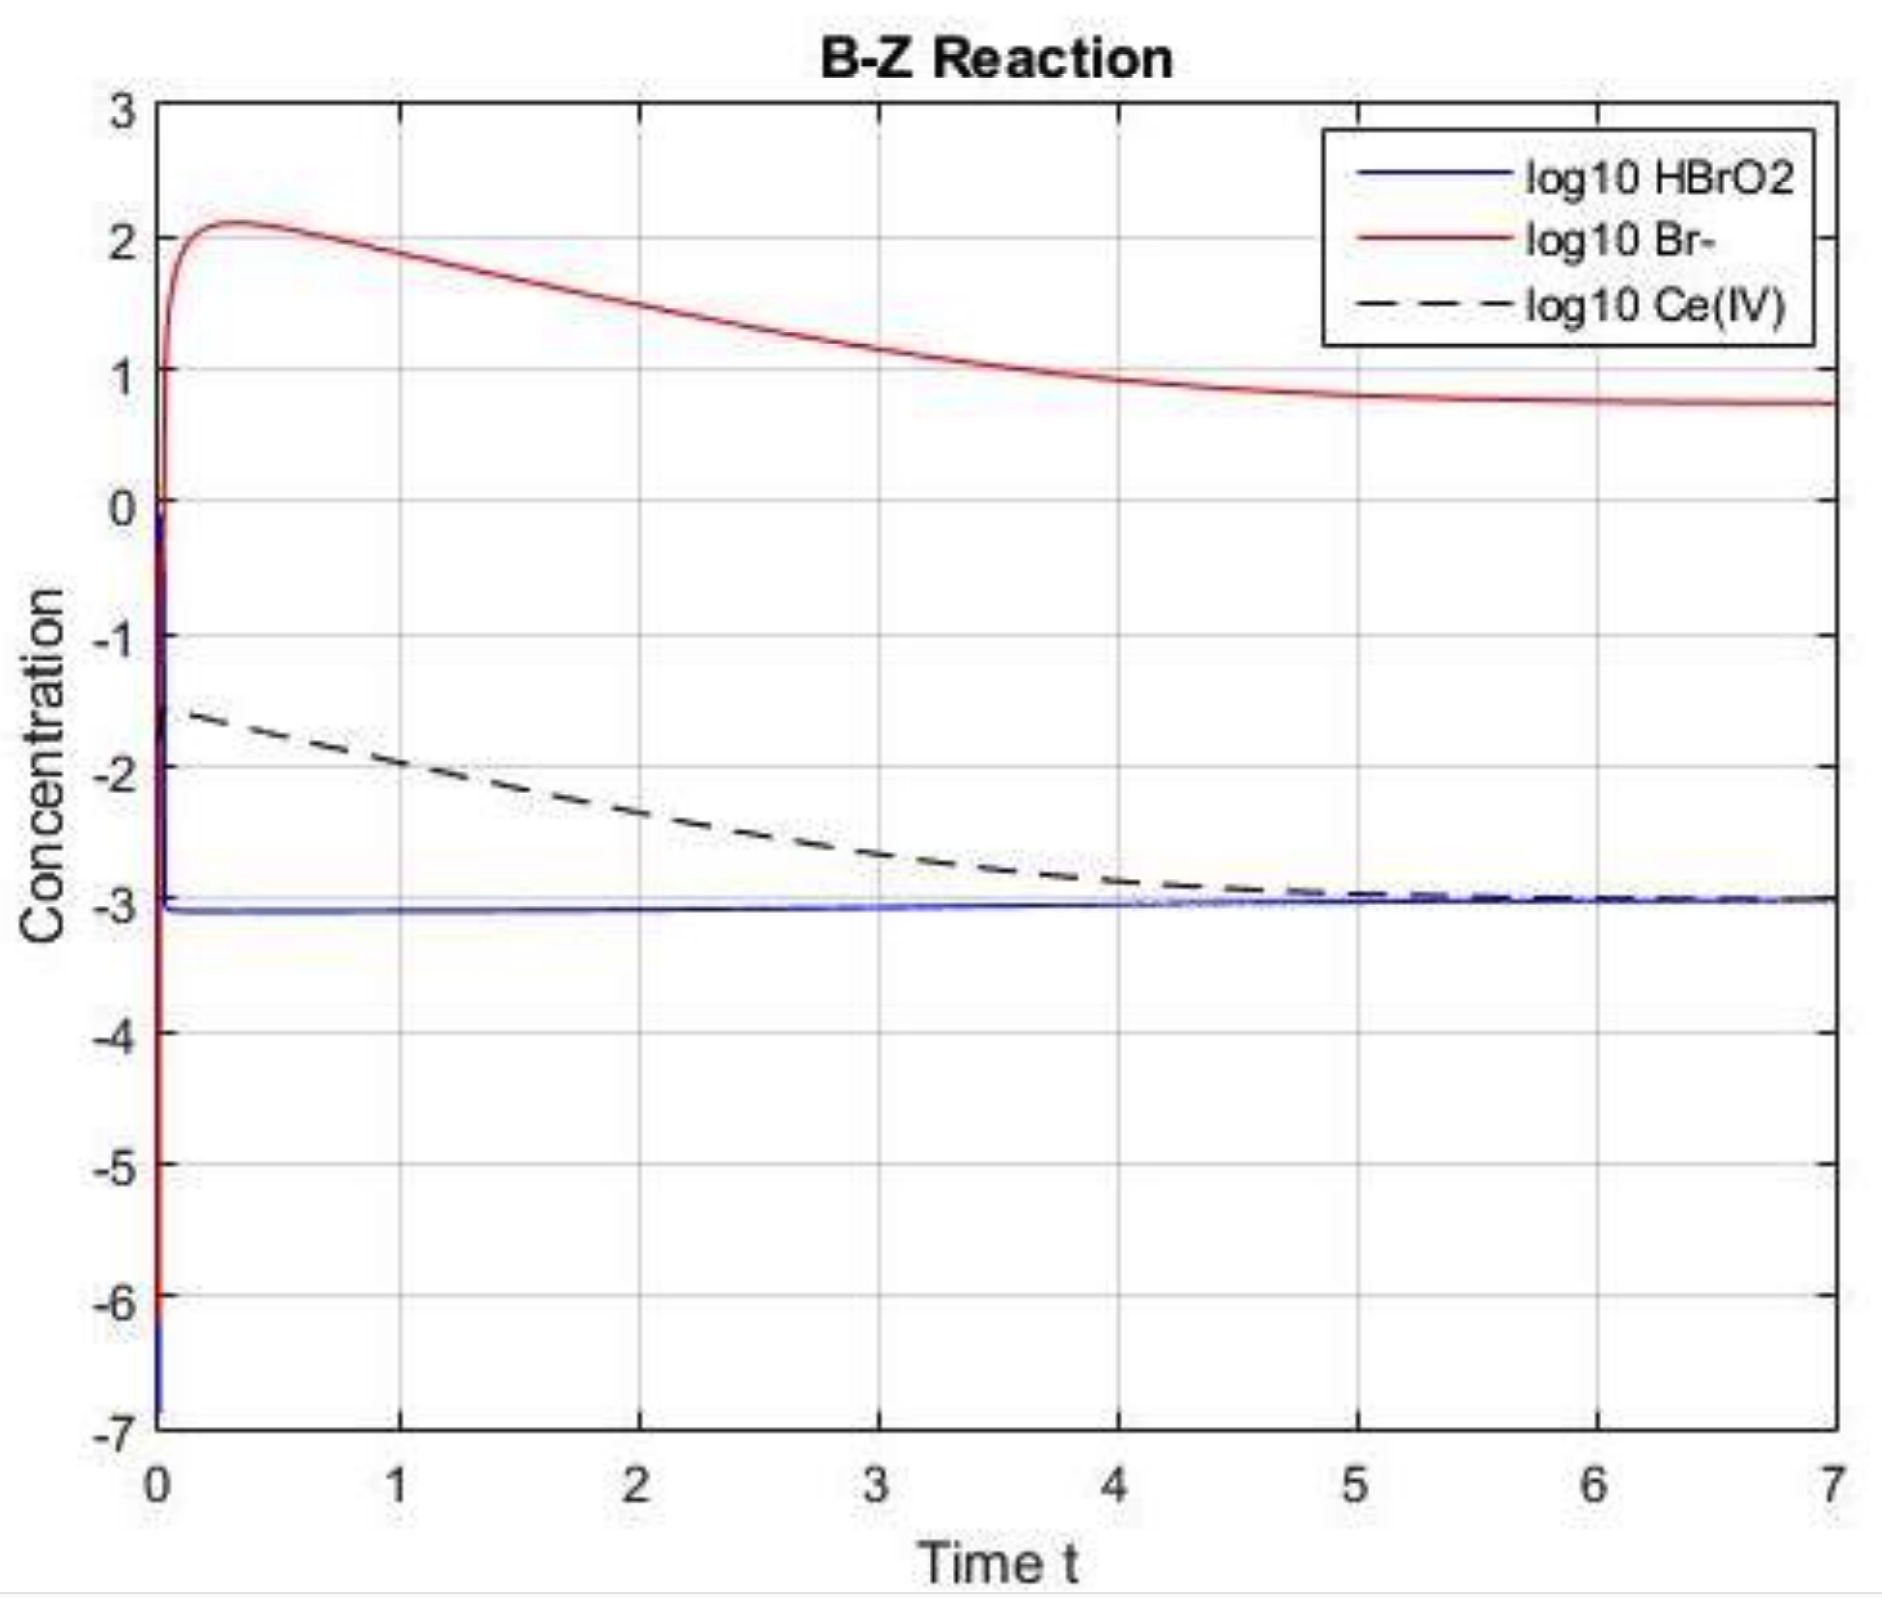
\includegraphics[width=0.3\linewidth]{pic/image.png}\\
        Gambar 2: Grafik $f = 0.1$
    \end{center} 
    \end{itemize}
\end{frame}

\begin{frame}{Simulasi dan Interpretasi}
     Diperhatikan bahwa pada $f = 0.1$, titik kesetimbangan dicapai saat $E_{2}^{*} =  (0.798, 0.2, 0.798)$ atau saat konsentrasi $x^* = [HBrO_2], z^* = [Ce(IV)] = 0.798 M$ dan $y^* = [Br^{-}] = 0.2 M$. Karena $f = 0.1 < 0.25$, maka reaksi stabil sebagaimana yang dapat dilihat pada Gambar 2.
\end{frame}

\begin{frame}{Simulasi dan Interpretasi}
    \begin{itemize}
    \item [2.] Untuk $f = 0.4$. Diperoleh grafik sebagai berikut: 
        \begin{center}
            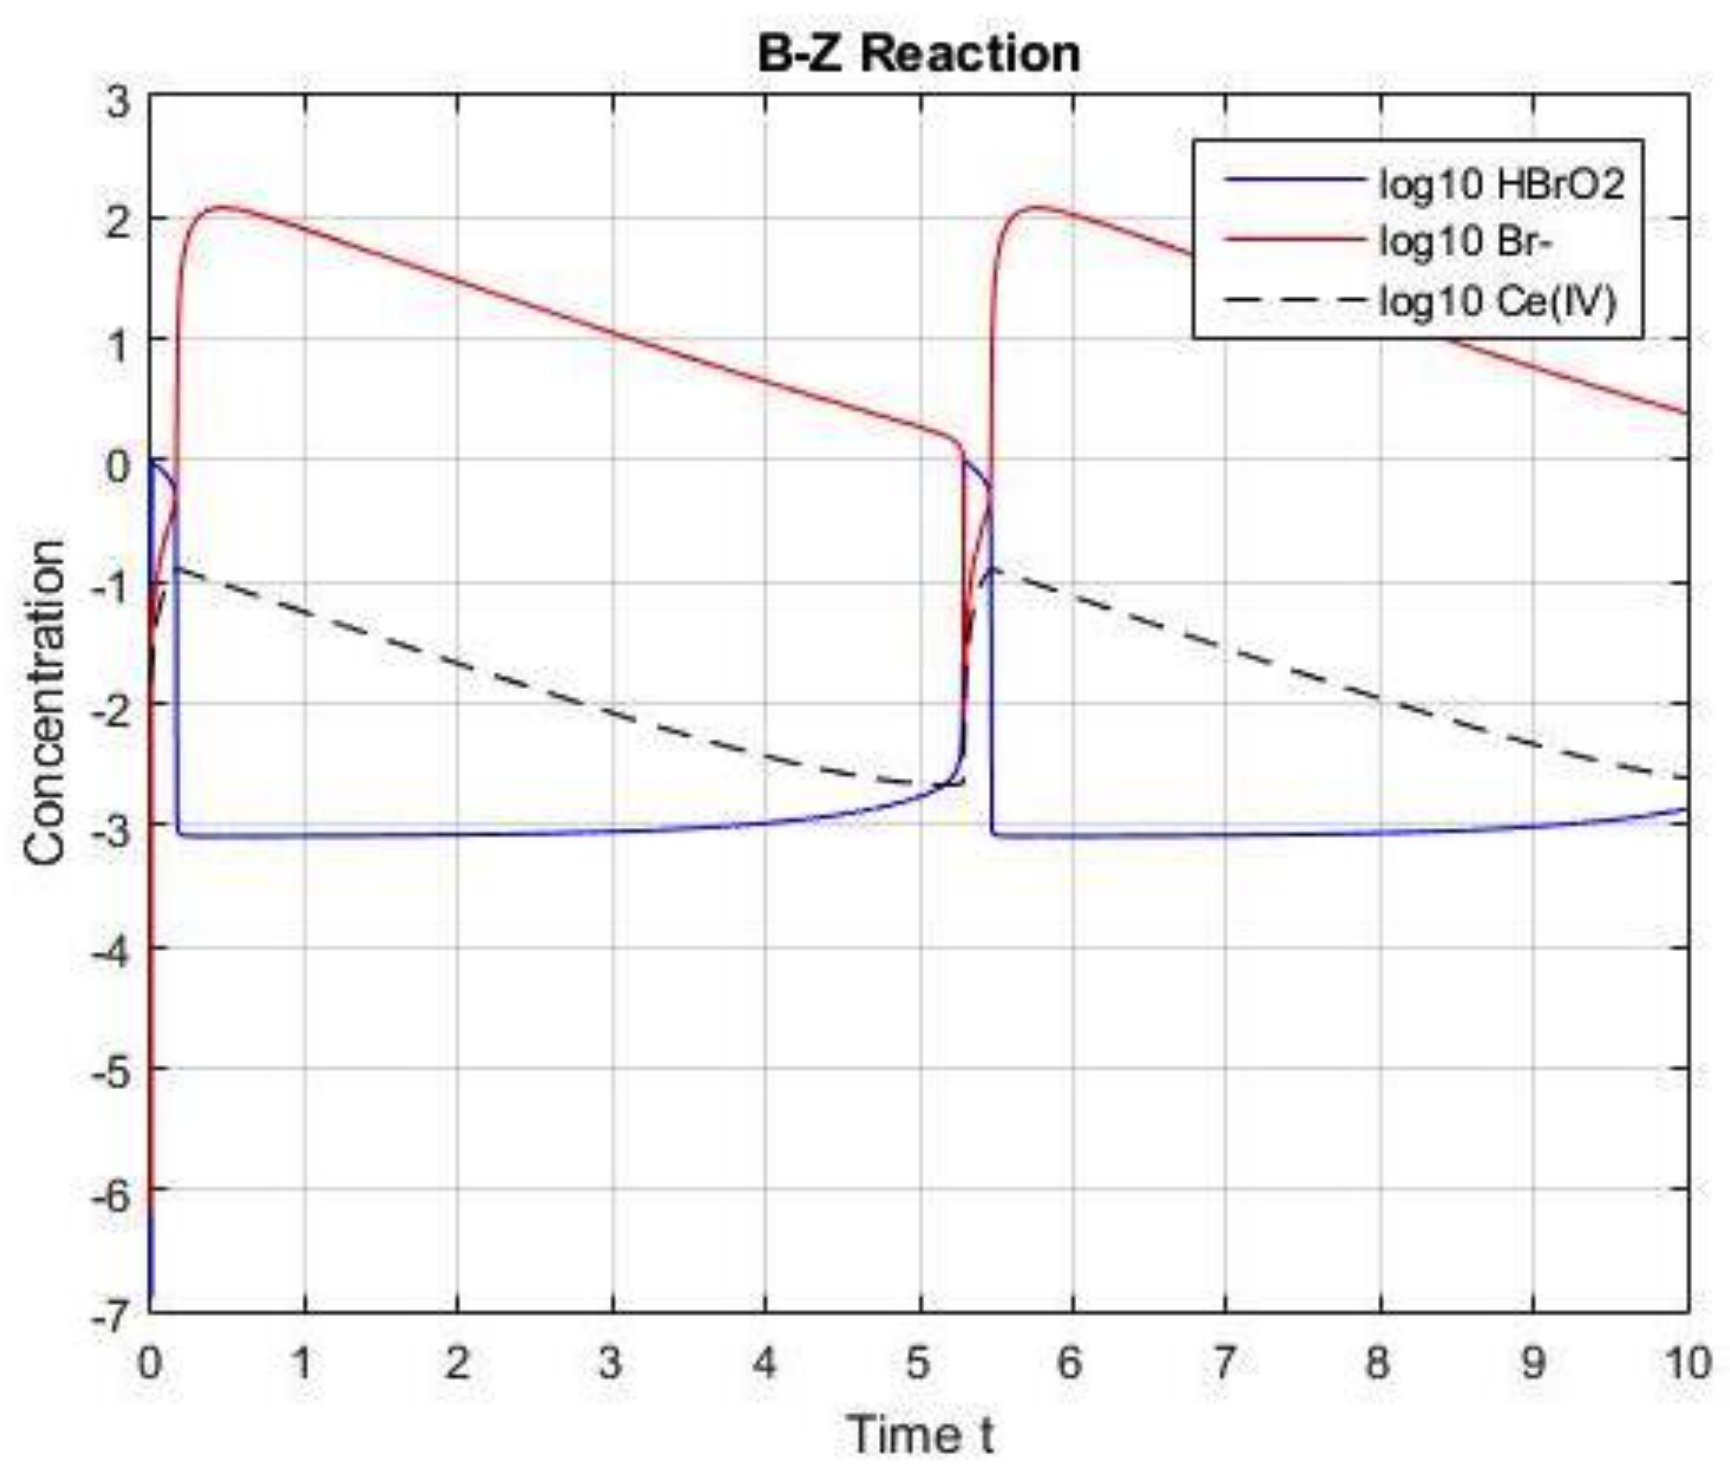
\includegraphics[width=0.3\linewidth]{pic/Screenshot 2024-06-22 at 17.02.48.png}\\
            Gambar 3: Grafik $f = 0.4$
        \end{center} 
    \end{itemize}
\end{frame}

\begin{frame}{Simulasi dan Interpretasi}
    Diperhatikan bahwa $0.25 < f = 0.4 < 0.5$ sehingga reaksi berosilasi dengan periode 
    $$T=\frac{2 \pi}{\sqrt{\frac{\left(q+x^*\right)\left(q+x^* 2\right.}{2 q \delta f+\delta x\left(q+x^*\right)+\varepsilon\left(q+x^*\right)\left(q+x^*+1\right)}}} = 6822.44.$$
    Konsentrasi $HBrO_2$, $Ce(IV)$, dan $Br^{-}$ naik dan turun secara berulang – ulang dan sistem tidak kunjung setimbang. Naik turunnya konsentrasi $HBrO_2$, $Ce(IV)$, dan $Br^{-}$ ini dapat diamati sebagai munculnya perubahan warna yang membentuk suatu pola pada reaksi saat eksperimen dilakukan. Akibatnya, pada $f = 0.4$, sistem tidak stabil.
\end{frame}

\section{Kesimpulan}
\begin{frame}{Kesimpulan}
    \begin{itemize}
    \item [1.] Terdapat dua titik setimbang dari Model Sistem Dinamik Oregonator Reaksi Belousov - Zhabotinsky, yaitu $E_1^*=(0,0,0)$ dan $E_2^*=(x^*,y^*,z^*)$, di mana 
        \begin{align}
        & x^* = \tfrac{1-f-q+\sqrt{1+q^2+4f^2+2q+12qf-4f}}{2}  \notag \\
        & y^* = \tfrac{2f(1-f-q+\sqrt{1+q^2+4f^2+2q+12qf-4f})}{1+q-f+\sqrt{1+q^2+4f^2+2q+12qf-4f}}  \notag \\
        & z^* = \tfrac{1-f-q+\sqrt{1+q^2+4f^2+2q+12qf-4f}}{2} \notag
        \end{align}
    dengan $1-2f-q>0$ dan $1+q^2+4f^2+2q+12qf-4f>0$.
     Titik setimbang $E_1^*=(0,0,0)$ tidak stabil dan titik setimbang $E_2^*=(x^*,y^*,z^*)$ terjadi bifurkasi
     \item [2.] Bifurkasi pada titik setimbang $E_2^*=(x^*,y^*,z^*)$ adalah bifurkasi Hopf dan sistem mengalami osilasi apabila nilai $f$ berada pada rentang $\tfrac{1}{4} < f < \tfrac{1}{2}$.
     \end{itemize}
\end{frame}

\section{Referensi}

\begin{frame}{Referensi}
    {Cd94} \hspace{0.5cm} M. S. Amelia, Apriliani E., Usadha I., \emph{Analisis Kestabilan dan Bifurkasi Model Oregonator dari Reaksi Belousov – Zhabotinsky}, JURNAL SAINS DAN SENI ITS \\ Vol. 8, No. 1 (2019).
\end{frame}

\begin{frame}
    \begin{center}
        {\Huge\calligra Terima kasih!}
    \end{center}
\end{frame}

\end{document}